\documentclass[12pt,oneside]{book} % use larger type; default would be 10pt

\usepackage[utf8]{inputenc} 
\usepackage[czech]{babel}
\usepackage[IL2]{fontenc}
\usepackage[a4paper]{geometry} 
\usepackage[pdftex]{graphicx} 
\usepackage[parfill]{parskip} 		% Activate to begin paragraphs with an empty line rather than an indent
\usepackage[explicit]{titlesec}
\usepackage{titletoc}
\usepackage{multirow}
\usepackage{bytefield}
\usepackage{rotating}
\usepackage{booktabs}  			% for much better looking tables
\usepackage{longtable}
\usepackage{lscape}
\usepackage{array} 	  		% for better arrays (eg matrices) in maths
\usepackage{paralist}  			% very flexible & customisable lists (eg. enumerate/itemize, etc.)
\usepackage{verbatim}  			% adds environment for commenting out blocks of text & for better verbatim
\usepackage{subfig}    			% make it possible to include more than one captioned figure/table in a single float
\usepackage[nottoc,notlof,notlot]{tocbibind} % Put the bibliography in the ToC
\usepackage[titles,subfigure]{tocloft}		 % Alter the style of the Table of Contents
\usepackage{color}
\usepackage[usenames,dvipsnames]{xcolor}
\usepackage{pdfmarginpar}
\usepackage{lastpage}
\usepackage{circuitikz}
\usepackage{tikz}
\usetikzlibrary{shapes,arrows,positioning,snakes,backgrounds,decorations.footprints,shadows,calc,chains} 
\usepackage{wrapfig}
\usepackage{listings}
\usepackage{tabularx}
\usepackage{enumitem}
\usepackage{anyfontsize}
\usepackage[pdftex, colorlinks=true, linkcolor=blue, urlcolor=blue]{hyperref} %should be last

\geometry{papersize={210mm,305mm},total={176mm,260mm}}

\usepackage{fancyhdr} % This should be set AFTER setting up the page geometry

\usepackage[local]{gitinfo2}

\pagestyle{fancyplain}     % options: empty , plain , fancy

\def\projectname{B5: Piano Tales Master}
\def\projectsubname{BROB - Základy robotiky\\[0.5cm]2019}
\def\projectdoc{Dokumentace projektu}

\definecolor{darkgray}{rgb}{0.4,0.4,0.9}
\definecolor{lightdarkgray}{rgb}{0.6,0.6,1.0}

\newcommand{\HRule}{\textcolor{darkgray}{\rule{\linewidth}{2mm}}}

\renewcommand{\headrulewidth}{1mm}
\renewcommand{\footrulewidth}{1mm}
\renewcommand{\plainheadrulewidth}{1mm}
\renewcommand{\plainfootrulewidth}{1mm}

\newcommand{\headrulecolor}{darkgray}
\newcommand{\footrulecolor}{darkgray}

\let\oldheadrule\headrule
\let\oldfootrule\footrule
\def\headrule{\textcolor{\headrulecolor}{\oldheadrule}}
\def\footrule{\textcolor{\footrulecolor}{\oldfootrule}}


\lhead{\projectdoc}
\chead{}
\rhead{\LARGE \projectname}
\lfoot{}
\cfoot{}
\rfoot{\thepage/\pageref{LastPage}}

\voffset 5mm
\setlength\headsep{8mm}

\newcommand{\up}[1]{\begin{sideways}\parbox{15mm}{#1}\end{sideways}}
\newcommand{\bx}[1]{\parbox{0.4\textwidth}{\centering #1}}

\tikzstyle{isipka} = [very thick,fill=none,rounded corners=2mm, color=red!100]
\tikzstyle{iodkaz} = [very thick,fill=none,rounded corners=3mm, color=red!100,line cap=round,align=center]
\tikzstyle{iprvek} = [rectangle, draw=red, rounded corners=3mm, line width=1mm]

\tikzstyle{postup} = [rectangle, draw, rounded corners=3mm, line width=1mm,minimum width=4cm,font=\bf]
\tikzstyle{labl} = [circle, draw, fill=white, rounded corners=3mm, line width=1mm,anchor=east,font=\bf]
\tikzstyle{edg} = [->, line width=1mm]

\tikzstyle{key} = [draw, fill=white, rectangle, rounded corners=2pt, inner sep=4pt, line width=0.5pt, drop shadow={shadow xshift=0.25ex,shadow yshift=-0.25ex,fill=black,opacity=0.75}, font=\scriptsize\sffamily, minimum height=1.5\baselineskip, minimum width=1.5\baselineskip]
\setcounter{secnumdepth}{-1}
\setcounter{tocdepth}{1}

\renewcommand\thepart{\arabic{part}}

\titleformat{\part}
  {\normalfont\normalsize}
  {}
  {20pt}
  {\begin{tikzpicture}[remember picture,overlay]%
	 \fill[lightdarkgray]  (current page.north west) rectangle ([yshift=-13cm]current page.north east);   
	 \node[fill=darkgray, text width=2\paperwidth, rounded corners=6cm, text depth=18cm, anchor=center, inner sep=0pt] at (current page.north east) (parttop) {\strut};
	 \node[anchor=south east, inner sep=0pt,	outer sep=0pt] at ([shift={(-2cm, +1cm)}]parttop.south)  (partnum) {\fontsize{10cm}{10}\selectfont\color{black}\thepart};
	 \node[anchor=north, inner sep=0pt]  at ([yshift=-2pt]partnum.south) (partname) {\large\scshape\bfseries\color{white} ČÁST};
 	 \node[anchor=north east, align=right, inner sep=0pt, outer ysep=2cm] at ([xshift=1cm]partnum.south) {\parbox{.7\textwidth}{\Huge\bfseries\raggedleft\projectname\\#1}};
 	 \node[anchor=north, align=left] at ([yshift=-12.5cm]current page.north) {\parbox{\textwidth}{\startcontents[part]\printcontents[part]{l}{0}{\setcounter{tocdepth}{0}}}};
   \end{tikzpicture}%    
  }

\titleformat{\chapter}
  {\normalfont}%
  {}%
  {20pt}%
  {\begin{tikzpicture}[remember picture,overlay]
    \fill[darkgray] (current page.north west) rectangle ([yshift=-3.5cm]current page.north east);
    \node[anchor=west, align=left, inner xsep=2cm] at ([yshift=-2cm]current page.north west) {\parbox{\textwidth}{\huge\sffamily\bfseries\scshape\color{white}#1}};%
   \end{tikzpicture}%
  }

\titlespacing*{\chapter}{0pt}{50pt}{-70pt}




\begin{document}
	
\begin{titlepage}
    \begin{center}

	~\\[0.5cm]
       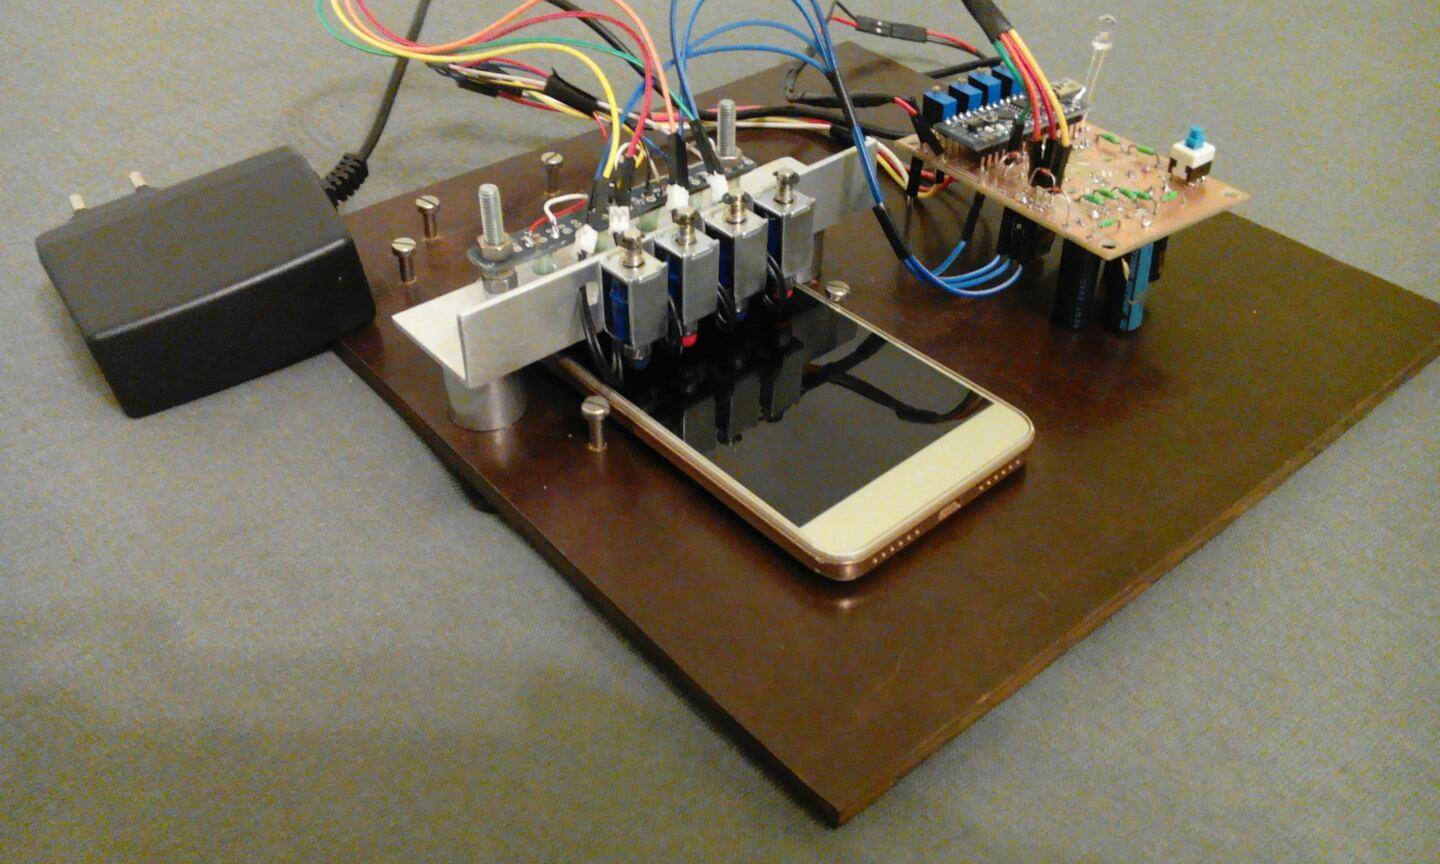
\includegraphics[width=0.85\textwidth]{./img/uvodka.jpg}\\[0cm] 

	~\\[2cm]

    % Title
    \HRule \\[0.4cm]
    { \huge \bfseries \projectname}\\[0.4cm]
       \textsc{\LARGE \projectsubname}\\[0.4cm]
    \HRule \\[1cm]
    
    \textsc{\LARGE \projectdoc}\\[0.5cm]
    \texttt{\Large \gitFirstTagDescribe}\\[1.5cm]

    % Author and supervisor
    \begin{minipage}{0.5\textwidth}
      \begin{center} \large
        
\includegraphics[width=0.85\textwidth]{./img/loga/vut.png}\\[1cm] 
		 \Large\bfseries UAMT FEKT VUT		
      \end{center}
    \end{minipage}%
    \begin{minipage}{0.5\textwidth}\raggedleft\Large\bfseries
 	Lukáš Zezula\par
        Dominik Řičánek\par
    \raggedright    
        Vedoucí projektu: \par
   \raggedleft     
        ing.Adam Ligocki
    \end{minipage}
    \vfill
   \end{center}
\end{titlepage}

\tableofcontents

%%%%%%%%%%%%%%%%%%%%%%%%%%%%%%%%%%%%%%%%%%%%%%%%%%%%%%%%%%%%%%%%%%%%%%%%%%%%%%%%%
%%%%%%%%%%%%%%%%%%%%%%%%%%%%%%%%%%%%%%%%%%%%%%%%%%%%%%%%%%%%%%%%%%%%%%%%%%%%%%%%%
%%%%%%%%%%%%%%%%%%%%%%%%%%%%%%%%%%%%%%%%%%%%%%%%%%%%%%%%%%%%%%%%%%%%%%%%%%%%%%%%%
%%%%%%%%%%%%%%%%%%%%%%%%%%%%%%%%%%%%%%%%%%%%%%%%%%%%%%%%%%%%%%%%%%%%%%%%%%%%%%%%%
\chapter{Analýza zadání}\label{analyza-zadani}
\section{Zadání}
\qquad Vytvořte robota, který bude hrát Piano Tales. Navrhněte stroj, který pomocí Vámi zvoleného HW (snímače a výpočetní jednotky a motorků) bude schopen hrát a porazit člověka ve hře Piano Tales. Referenčním výsledkem bude https://www.youtube.com/watch?v=fqOW84ZTL7k který se pokusíme porazit. Na závěr vznikne krátké propagační video na youtube obsahujcí logo VUT.
Projekt bude veden pomoci GITu. Dokumentace bude vytvořená v LaTeXu. 
\section{Úvod}\label{uvod}
\qquad Cílem projektu, jak je patrno ze zadání, bylo realizovat robota, který by hrál hru Piano Tales a dosahoval lepších výsledků než člověk a ideálně se přiblížil, nebo dokonce překonal referenční výsledek.

\qquad Hra Piano Tales funguje tak, že po obrazovce ve čtyřech lajnách jezdí obdélníky, jejichž stisknutím se zvýší skóre a rychlost s jakou se pohybují. Hra se tedy neustále ztěžuje. Jakmile nezachytíte již zmiňovaný obdélník nebo kliknete mimo jeho plochu, hra končí. Krom těchto obdélníků, které mají pevně definované rozměry, jezdí po obrazovce i delší obdélníkové úseky, které mají stálou šířku, ale jejich délka se různí (viz. Obrázek \ref{pianotales}). Tyto úseky se liší i barevně. Zatímco obdélníky jsou vždy striktně černé, tak barva úseků se mění od černé na začátku úseku po světlejší odstíny modré na konci. Přidržením těchto úseků od počátku do konce se skóre zvýší více než při pouhém stisknutí. 

\begin{figure}[ht] \large\centering
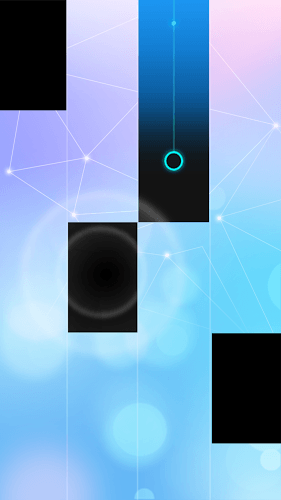
\includegraphics[width=0.30\textwidth]{./img/pianotales.png}\\[1cm] 
\caption{Ukázka hrací plochy hry Piano Tales}
\label{pianotales}
\end{figure}   
      
\section{Nástin řešení}\label{nastin}
\qquad Oproti videu, přiloženému k zadání, jsme neměli k dispozici tablet, kolem kterého by se dali pohodlně rozmístit servomotory, a proto jsme museli použít smartphone, který má podstatně menší rozměry. Toto vedlo na nutnost pracovat s menšími prvky, které by ovládaly dotykový display a složitější mechanickou konstrukci.

\qquad Nejvhodnější se ukázalo použití elektromagnetů, konkrétně push type solenoidů, které byly pomocí mechanické konstrukce umístěny nad smartphonem tak, aby po přivedení napětí na řídící obvod stiskly specifické místo na dotykovém displayi.

\qquad Ke snímání průběhů obdélníků byly použiti fotorezistory. Ty byly umístěny dostatečně blízko displaye a ve speciálně vytvořeném pouzdru, aby se minimalizoval vliv okolního osvětlení. 

\qquad Zjednodušený princip, s jakým výsledný robot hraje hru, lze vidět na Obrázku \ref{blok_0}. Obdélník, mající černou barvu, se pohybuje po světle modrém pozadí kolem fotorezistoru. To zapříčiní změnu odporu, kterou zachycuje mikroprocesor a měří čas mezi přechody modrá-černá, černá-modrá. Z tohoto času a známých rozměrů obdélníku se vypočte rychlost, s kterou se obdélník pohybuje. Po započítání dopravního zpoždění, které je dáno zejména časem potřebným k sepnutí solenoidu, se určí okamžik, kdy přesně má být přiveden z mikroprocesoru spínací signál na vstup řídícího obvodu.

\begin{figure}[ht] \large\centering
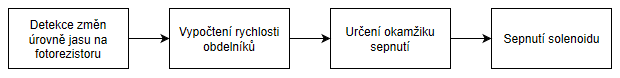
\includegraphics[width=0.80\textwidth]{./img/blok_0.png}\\[1cm] 
\caption{Zjednodušený princip funkce robotu}
\label{blok_0}
\end{figure}   
%%%%%%%%%%%%%%%%%%%%%%%%%%%%%%%%%%%%%%%%%%%%%%%%%%%%%%%%%%%%%%%%%%%%%%%%%%%%%%%%%
%%%%%%%%%%%%%%%%%%%%%%%%%%%%%%%%%%%%%%%%%%%%%%%%%%%%%%%%%%%%%%%%%%%%%%%%%%%%%%%%%
%%%%%%%%%%%%%%%%%%%%%%%%%%%%%%%%%%%%%%%%%%%%%%%%%%%%%%%%%%%%%%%%%%%%%%%%%%%%%%%%%
%%%%%%%%%%%%%%%%%%%%%%%%%%%%%%%%%%%%%%%%%%%%%%%%%%%%%%%%%%%%%%%%%%%%%%%%%%%%%%%%%
\part{MECHANICKÁ ČÁST}\label{mechanika}
\chapter{Návrh v prostředí AutoCAD}\label{CAD}

\begin{figure}[ht]\large\centering
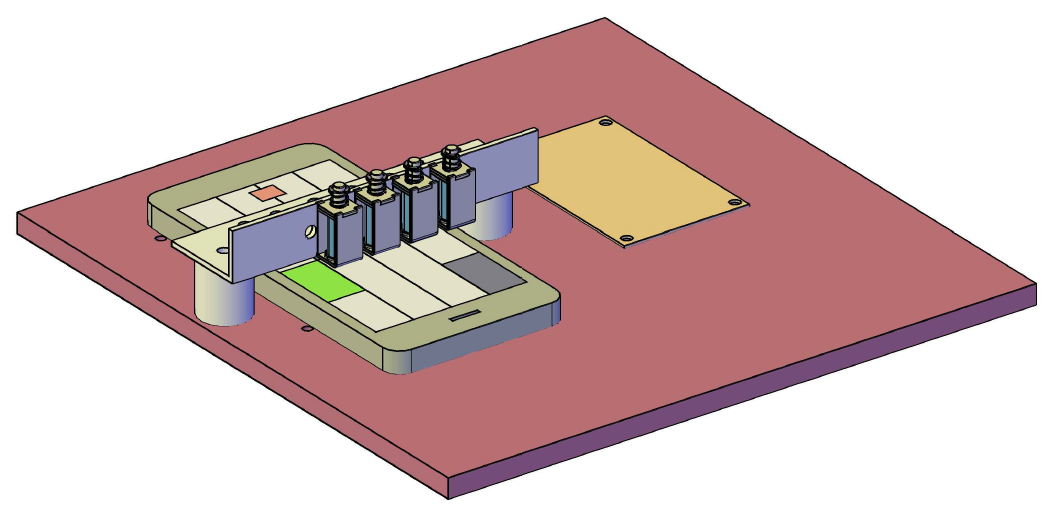
\includegraphics[width=1.00\textwidth]{./img/mech_cad0.png}\\[1cm] 
\caption{Model mechanické části v prostředí AutoCAD jiho-západní pohled}
\label{mech_cad0}
\end{figure}  

\begin{figure}[ht]\large\centering
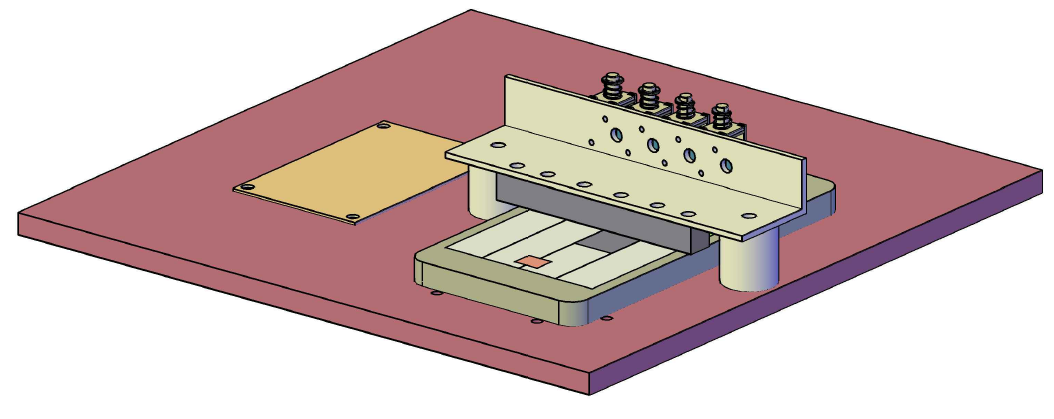
\includegraphics[width=1.00\textwidth]{./img/mech_cad1.png}\\[1cm] 
\caption{Model mechanické části v prostředí AutoCAD severo-západní pohled}
\label{mech_cad1}
\end{figure}  

\pagebreak

\section{Popis částí modelu}\label{mech_casti}
\qquad Model byl pomyslně rozdělen na 5 částí. Konkrétně se jedná o podstavu, L-profil, válcové spojky, solenoidy a pouzdro na fotorezistory. Tyto části jsou navrženy tak, aby byly demontovatelné (spoje jsou realizovány pouze šrouby a případně maticemi). Jak na sebe jednotlivé části navazují můžeme vidět na Obrázku \ref{mech_cad0} a \ref{mech_cad1}. Oranžový obdélníkový profil představuje plošný spoj.

\textbf{podstava}

\qquad Uchycením všech částí konstrukce pevně na podstavu čtvercového tvaru jsme předešli nežádoucím posuvům a docílili větší stability konstrukce. Více o nákresu a rozměrech podstavy viz. Příloha \hyperref[Prilohy]{1}.

\textbf{L-profil}

\qquad Tento profil ukotvuje solenoidy a pouzdro na fotorezistory. Je připevněn na válcové spojky, aby byl ve správné výšce nad smartphonem. Náčrt L-profilu lze vidět na Obrázku \ref{lprof}. Více o nákresu a rozměrech L-profilu viz. Příloha \hyperref[Prilohy]{1}.  

\begin{figure}[ht] \large\centering
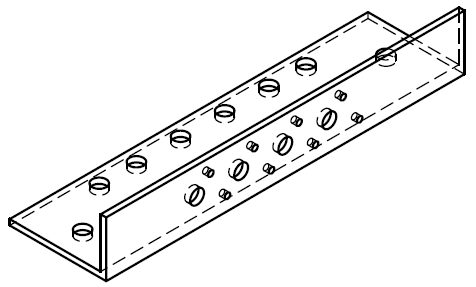
\includegraphics[width=0.60\textwidth]{./img/lprof.png}\\[1cm] 
\caption{Náčrt L-profilu}
\label{lprof}
\end{figure}   

\textbf{válcové spojky}

\qquad Jejich hlavní funkce spočívá v přichycení L-profilu k podstavě ve správné výšce tak, aby při sepnutí solenoidu došlo k interakci stylusů, umístěných na solenoidech, s dotykovým displayem. Rozměry válcových spojek byly tedy voleny tak, aby při zahrnutí tloušťky smartphonu (cca 9mm), výšky stylusu (cca 9,5mm) a zdvihu solenoidu (cca 3.5mm) došlo po přivedení napětí k již zmíněnému dotyku.  Více o nákresu a rozměrech válcových spojek viz. Příloha \hyperref[Prilohy]{1}.


\textbf{solenoidy}

\qquad Jak již bylo zmíněno v \hyperref[nastin]{Nástinu řešení} museli být použity součástky, které by se dali umístit kolem poměrně malého smartphonu. Pro tento účel jsme vybrali push type solenoidy se zdvihem okolo 3.5mm a rozměry takovými, aby se na šířku smartphonu (cca 74mm) vlezly alespoň 4 tyto solenoidy. Konkrétní rozměry solenoidů lze vyčíst z datasheetu viz. Příloha \hyperref[Prilohy]{4}. 3D model solenoidu byl převzat ze stránek GRABCAD COMMUNITY. \cite{grabcad}

\pagebreak
\textbf{pouzdro na fotorezistory}

\qquad Jeho hlavní význam spočívá v odstínění okolního osvětlení a ukotvení fotorezistorů na požadované místo. Je přichyceno k L-profilu a umístěno v takové výšce nad smartphonem, aby fotorezistory dostatečně dobře snímaly změny jasu na displayi a zároveň nebyly příliš ovlivněny osvětlením místnosti. Fotorezistory jsou v pouzdru zapuštěny cca 1mm a jsou vzdáleny od smartphonu cca 4mm. Náčrt pouzdra lze vidět na Obrázku \ref{pouzdro}. Více o nákresu a rozměrech pouzdra na fotorezistory viz. Příloha \hyperref[Prilohy]{1}.

\begin{figure}[ht] \large\centering
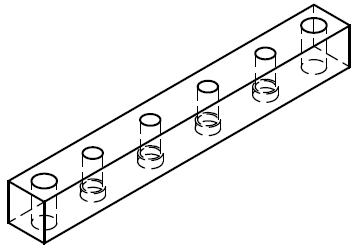
\includegraphics[width=0.60\textwidth]{./img/pouzdro.png}\\[1cm] 
\caption{Náčrt pouzdra na fotorezistory}
\label{pouzdro}
\end{figure}  

\chapter{Konstrukce mechanické části}\label{konstr}
\qquad Všechny části konstrukce byly nařezány, obroušeny a byly do nich navrtány díry a závity dle výkresové dokumentace (viz. Příloha \hyperref[Prilohy]{1}).

\qquad Jako materiál pro podstavu byl zvolen akryl, hlavně díky jeho dostupnosti a kvalitním izolačním vlastnostem. Závity, které se nacházejí kolem smartphonu a lze je vidět na Obrázku \ref{mech_cad0} a \ref{mech_cad1}, slouží pro šrouby M4, které nebyly zašroubovány na doraz proto, aby se mezi ně dal zasunout smartphone a tím byl pevně uchycen na jedno místo. K podstavě byla přišroubována deska plošných spojů.

\qquad Válcové spojky a L-profil byly odříznuty z hliníkových profilů (konkrétně typ AlMgSi0,5). K válcovým spojkám je z jedné strany šroubem M5 přišroubovaná podstava a z druhé L-profil. K L-profilu je poté pomocí šroubů M5 a matic přichyceno pouzdro na fotorezistory a tyto jsou připájeny na kousek univerzálního pájivého pole, odkud potom vedou dráty na plošný spoj. 

\qquad Do rámu solenoidů byly do předchystaných děr vyřezány závity M2 a následně jsme solenoidy přišroubovali k L-profilu.Napájecí kabely solenoidů jsme protáhli příslušnými dírami a přivedli na desku plošných spojů. Stylusy byly, vzhledem k jejich malým rozměrům a faktu, že by nevydržely obrábění, k solenoidům přilepeny tekutým kovem (WURTH tekutý kov FE1).

\qquad Na závěr bylo nutné zajistit, aby se přívodní drátky fotorezistorů nemohly dotknout hliníkového L-profilu. Toho bylo dosaženo umístěním odstřižků plastových slámek kolem zmíněných drátků. 

\qquad Vybrané snímky z konstrukce mechanické části lze vidět na Obrázku \ref{konstr0} a \ref{konstr1}

\begin{figure}[ht] \large\centering
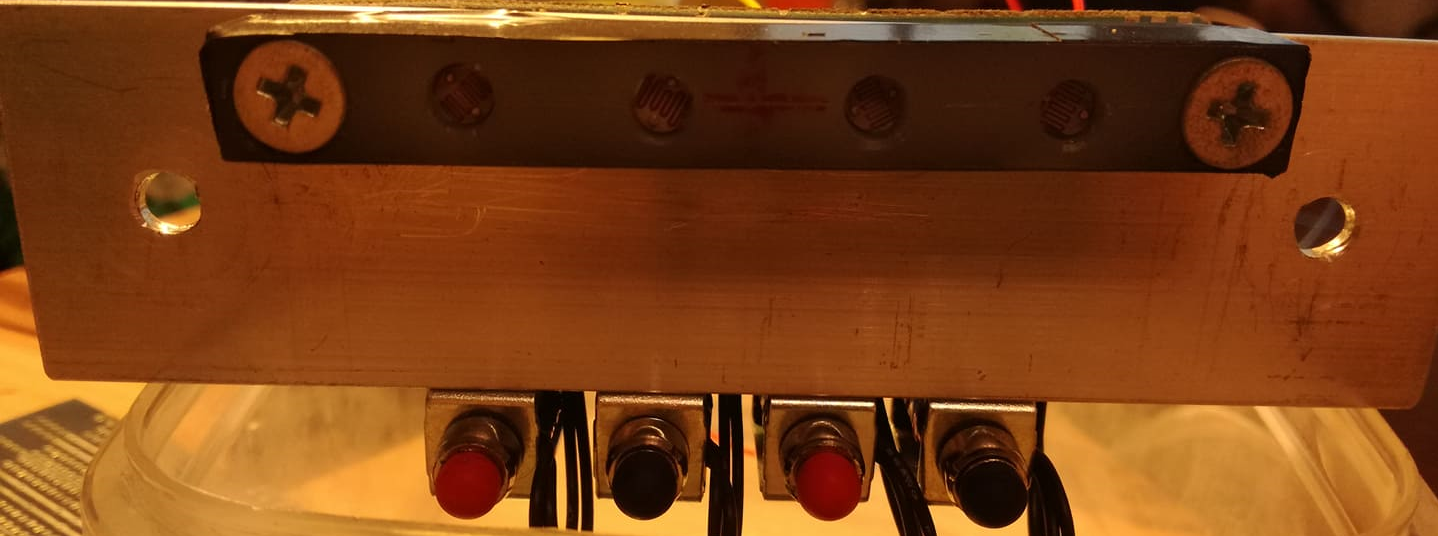
\includegraphics[width=0.80\textwidth]{./img/konstr0.png}\\[1cm] 
\caption{Fotka spodní části L-profilu s přichycenými solenoidy a pouzdrem na fotorezistory}
\label{konstr0}
\end{figure} 

\begin{figure}[ht] \large\centering
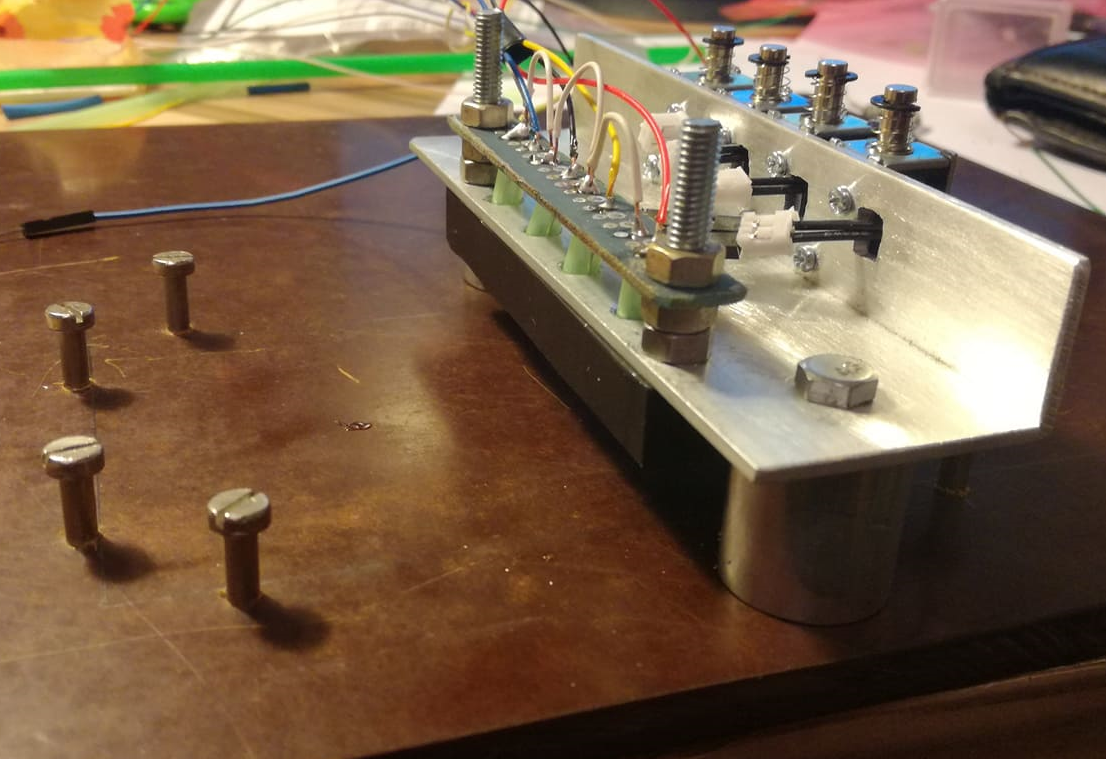
\includegraphics[width=1.00\textwidth]{./img/konstr1.png}\\[1cm] 
\caption{Fotka mechanické konstrukce - severo-západní pohled}
\label{konstr1}
\end{figure} 
%%%%%%%%%%%%%%%%%%%%%%%%%%%%%%%%%%%%%%%%%%%%%%%%%%%%%%%%%%%%%%%%%%%%%%%%%%%%%%%%%
%%%%%%%%%%%%%%%%%%%%%%%%%%%%%%%%%%%%%%%%%%%%%%%%%%%%%%%%%%%%%%%%%%%%%%%%%%%%%%%%%
%%%%%%%%%%%%%%%%%%%%%%%%%%%%%%%%%%%%%%%%%%%%%%%%%%%%%%%%%%%%%%%%%%%%%%%%%%%%%%%%%
%%%%%%%%%%%%%%%%%%%%%%%%%%%%%%%%%%%%%%%%%%%%%%%%%%%%%%%%%%%%%%%%%%%%%%%%%%%%%%%%%
\part{ELEKTRONICKÁ ČÁST}\label{elektro}

\chapter{Úvod}\label{uvodelektro}
\qquad Schéma celé elektronické části projektu lze vidět na Obrázku \ref{schematic}. Elektronickou část lze pomyslně rozdělit na dva samostatné obvody: snímací a řídící. Elektronická část je napájena spínaným napěťovým zdrojem 12V/2A a jako řídící jednotka je použito Arduino nano. Jak můžeme vidět na pinu D12, je připojeno tlačítko, sloužící k zahájení hry.

\qquad \textbf{Snímací obvod} slouží k zachycení změn jasu na fotorezistoru. Princip jeho funkce je velice jednoduchý. Fotorezistor tvoří s potenciometrem odporový dělič, na který je přivedeno 5,5V napětí z Arduina. Jakmile pod fotorezistorem probíhá černý obdelník na displayi smartphonu, jeho odpor, důsledkem snížení intenzity dopadajícího světla, vzroste. To zapříčiní vzrůst úbytku napětí na fotorezistoru, který měří AD převodník Arduina. Naopak při průběhu světle modrého pozadí pod fotorezistorem je intenzita dopadajícího světla větší, což zapříčiní snížení odporu fotorezistoru. Důsledkem toho na něm úbytek napětí poklesne. Jelikož byly použity levné fotorezistory, které nemají garantované průběhy odporu v závislosti na intenzitě světla, musí být výsledné napěťové děliče nastaveny na přibližně stejné výstupní hodnoty napětí pomocí potenciometrů.

\qquad\textbf{Řídícím obvodem} se budeme zabývat v následující části textu.

\begin{figure}[ht] \large\centering
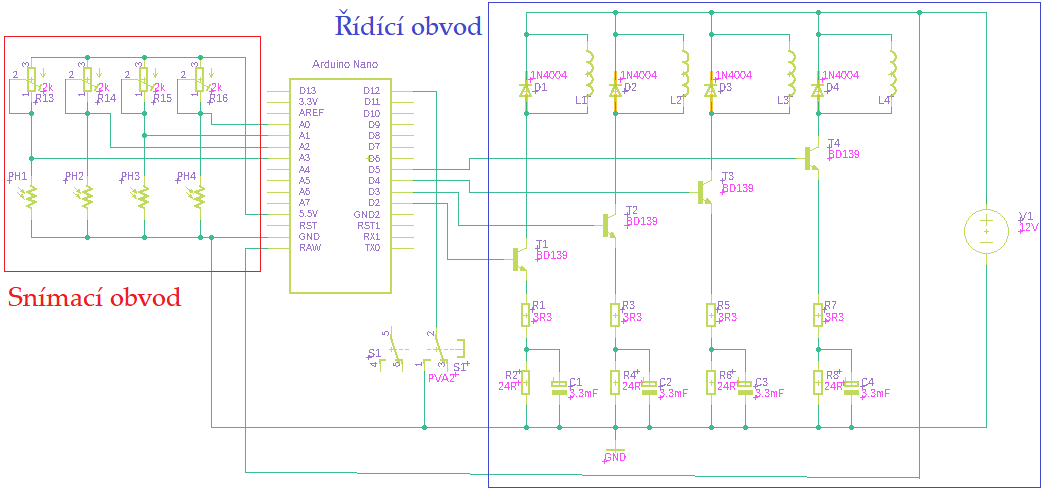
\includegraphics[width=1.00\textwidth]{./img/schematic.png}\\[1cm] 
\caption{Schéma celé elektronické části projektu}
\label{schematic}
\end{figure} 

\chapter{Návrh řídícího obvodu}\label{ridiciobvod}
\section{Solenoid}\label{solenoid_elektro}
\qquad Solenoid je v podstatě cívka, což znamená, že má nějaký odpor vinutí a indukčnost. Odpor vinutí udává výrobce jako 4,5$\Omega$ a rovněž udává napětí potřebné k sepnutí jako 5V a proud tekoucí solenoidem jako 1,1A (více informací lze získat z datasheetu viz. Příloha \hyperref[Prilohy]{4}). Změřili jsme však, že tyto podmínky jsou značně předimenzované. Skutečný proud při kterém solenoid sepne byl vyhodnocen ze série měření jako 400mA, což ovšem vedlo ke snížení rychlosti sepnutí. Proud, při kterém solenoid rozepne, byl 50mA. Z tohoto měření vyplynul zajímavý poznatek. Proud, který je potřeba k sepnutí solenoidu, je mnohem větší než ten, který je potřeba k udržení solenoidu v sepnutém stavu. Výrobce bohužel neudává indukčnost solenoidu, tak byla orientačně změřena jako 2,2uH. Základní představy o principu funkce solenoidu byly převzaty z článku na stránkách SCIENCING. \cite{solenoid_bib}

\section{Požadavky na řídící obvod}\label{pozadavky}
\qquad V požadavcích na řídící obvod je zřejmý technický rozpor. Potřebujeme spínat indukčnost dostatečně rychle, aby byl obvod použitelný i pro pozdější fáze hry, ale to vede na nepříjemné zvýšení proudu. Vzhledem k tomu, že máme k dispozici pouze zdroj s maximálním proudem 2A znamenalo by to, že by jsme v jednu chvíli mohli ovládat pouze jeden, maximálně dva solenoidy. Toto je pro praktickou funkčnost naprosto nepřípustné.

\qquad Řešení tohoto problému vedlo na separaci v čase, kdy pro sepnutí solenoidu pustíme do obvodu velkou proudovou špičku (cca 1A) a poté udržujeme stálou hodnotu proudu (cca 150mA) pro udržení solenoidu v sepnutém stavu. Nejjednodušší, a hlavně nejlevnější, možností jak toho dosáhnout bylo využití přechodových dějů v obvodu.

\section{Návrh v prostředí Matlab Simulink}\label{matsim}
Výsledný návrh řídícího obvodu pro spínání solenoidu můžeme vidět na Obrázku \ref{schema0}. Po připojení napájecího napětí (12V) se obvod, velmi zjednodušeně řečeno, chová jako proudový zdroj.

\qquad Po přivedení napětí z Arduina mezi bázi tranzistoru a zem má tendenci téct proud. Skokové změny proudu na cívce nelze dosáhnout, ale vzhledem k malé indukčnosti solenoidu proud roste po velmi strmé exponenciále. Pomalu se začíná nabíjet kondenzátor, který má poměrně velkou kapacitu, což zapříčiňuje exponenciální klesání proudu až na ustálenou hodnotu (cca 150mA). Tímto způsobem byla vytvořena proudová špička, která zapříčiní sepnutí solenoidu, a následná ustálená hodnota proudu udržuje solenoid v sepnutém stavu.

\qquad Pokud odpojíme napětí, přivedené mezi bázi a zem, tranzistorem přestává téct proud a indukčnost má tendenci vytvořit napěťovou špičku. Z toho důvodu je k ní antiparalelně zavedena usměrňovací dioda, která zabrání překročení napětí 0,6V. Kondenzátor se vybíjí přes odpor do země.

\quad Výsledné průběhy můžeme vidět na Obrázku \ref{prubehy}. Pro datasheet k použitému tranzistoru viz. Příloha \hyperref[Prilohy]{4}. Pro simulační schéma v Simulinku a matlabovský spouštěcí skript viz. Příloha \hyperref[Prilohy]{3}.

\begin{figure}[ht] \large\centering
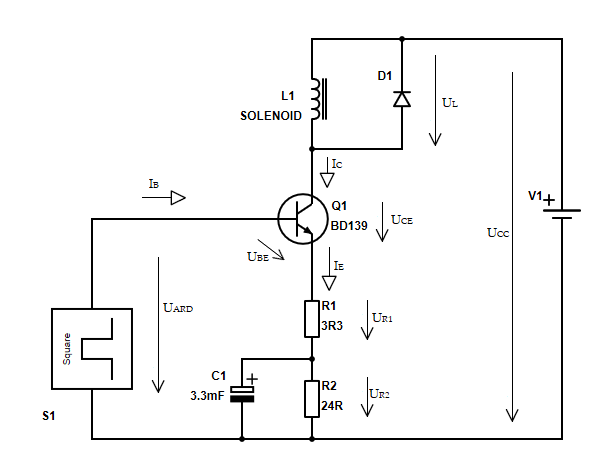
\includegraphics[width=0.60\textwidth]{./img/schema0.png}\\[1cm] 
\caption{Schéma řídícího obvodu pro spínání solenoidu}
\label{schema0}
\end{figure} 

\begin{figure}[ht] \large\centering
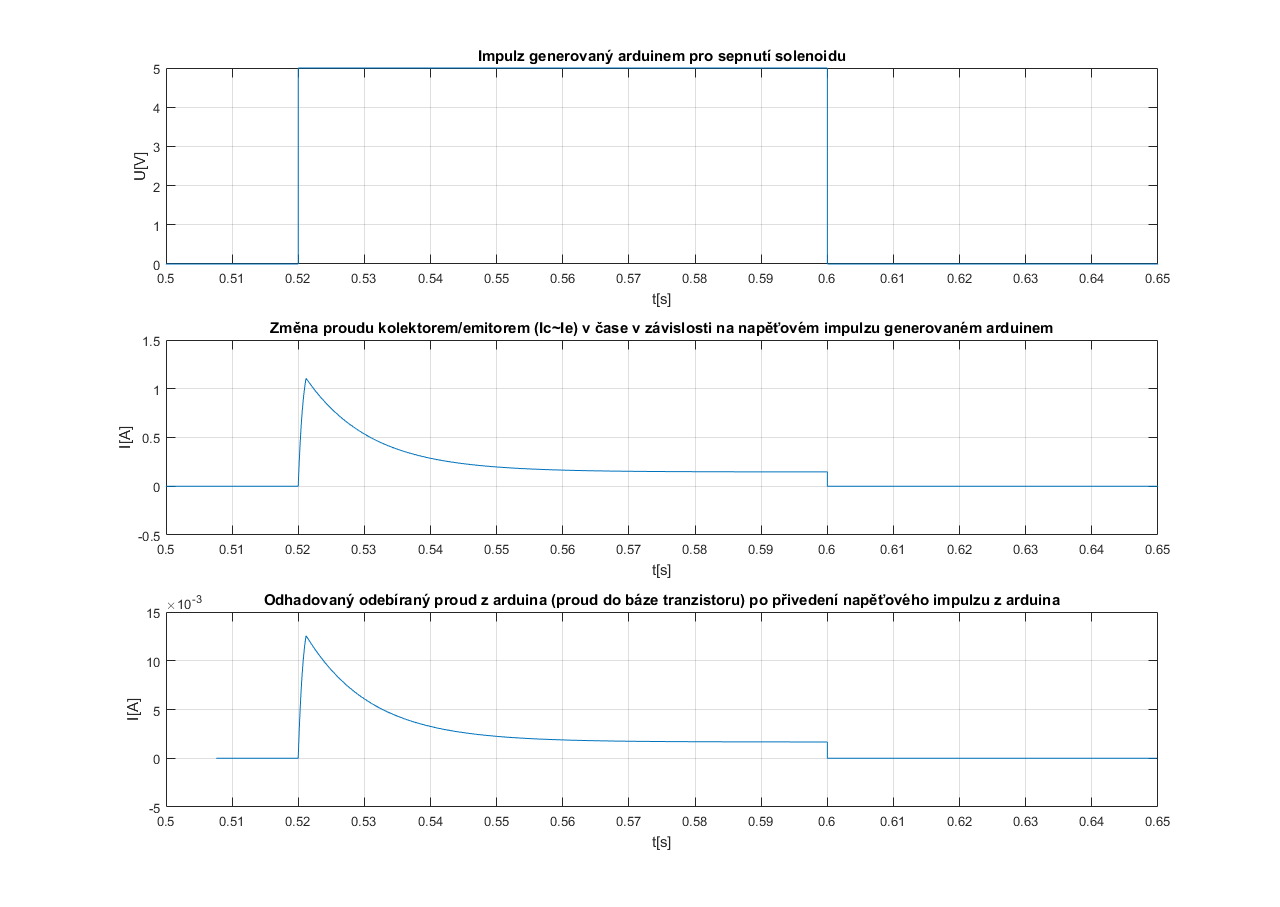
\includegraphics[width=1.00\textwidth]{./img/prubehy.png}\\[1cm] 
\caption{Průběhy proudů řídícího obvodu v čase vytisknuté z Matlabu}
\label{prubehy}
\end{figure} 

\chapter{Měření obvodových veličin v řídícím obvodu}\label{mer_elektro}
\section{Ustálené stavy obvodových veličin}
\qquad Následující odstavec dává přehled o hodnotách, na kterých se ustálí obvodové veličiny po odeznění přechodových dějů při přivedení napětí z Arduina mezi bázi a zem. Můžeme uvažovat zjednodušené schéma viz. Obrázek \ref{schema1}. Hodnoty byly naměřeny ručním multimetrem dostupným v laboratoři robotiky.
\begin{figure}[ht] \large\centering
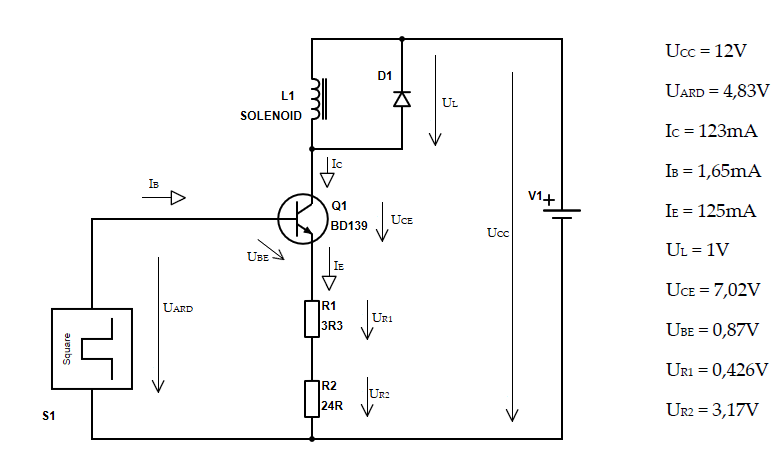
\includegraphics[width=0.50\textwidth]{./img/schema1.png}\\[1cm] 
\caption{Schéma řídícího obvodu simulující ustálené hodnoty obvodových veličin}
\label{schema1}
\end{figure} 

\section{Měření maximálních hodnot obvodových veličin}
\qquad Následující odstavec dává přehled o hodnotách, kterých dle daného zapojení (viz. Obrázek \ref{schema0}) dosahují obvodové veličiny v extrému. Podstatná pro nás je zejména hodnota proudu odebíraného z Arduina, která nesmí překročit 20mA. Můžeme uvažovat zjednodušené schéma dávající přehled o maximálních hodnotách viz. Obrázek \ref{schema2}.

\begin{figure}[ht] \large\centering
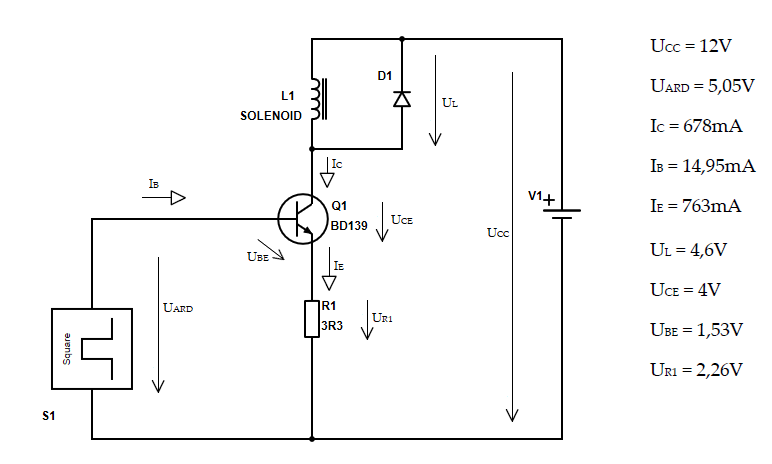
\includegraphics[width=0.50\textwidth]{./img/schema2.png}\\[1cm] 
\caption{Schéma řídícího obvodu simulující maximální hodnoty obvodových veličin}
\label{schema2}
\end{figure} 

\chapter{Deska plošných spojů}\label{elektro_deska}
\qquad Návrh desky plošných spojů byl proveden v prostředí Eagle (viz. Příloha \hyperref[Prilohy]{2}) dle návodu uvedeném na webu předmětu Robotika \cite{robotika}. Návrh můžeme také vidět na Obrázku \ref{pcb}

\begin{figure}[ht] \large\centering
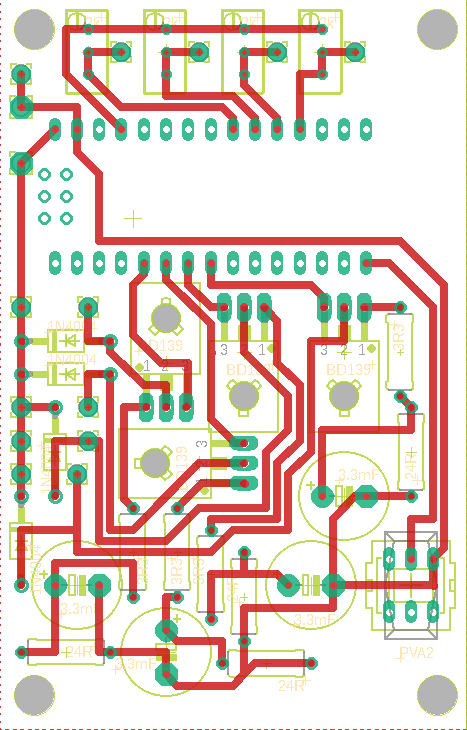
\includegraphics[width=0.60\textwidth]{./img/pcb.png}\\[1cm] 
\caption{Návrh desky plošných spojů}
\label{pcb}
\end{figure} 
%%%%%%%%%%%%%%%%%%%%%%%%%%%%%%%%%%%%%%%%%%%%%%%%%%%%%%%%%%%%%%%%%%%%%%%%%%%%%%%%%
%%%%%%%%%%%%%%%%%%%%%%%%%%%%%%%%%%%%%%%%%%%%%%%%%%%%%%%%%%%%%%%%%%%%%%%%%%%%%%%%%
%%%%%%%%%%%%%%%%%%%%%%%%%%%%%%%%%%%%%%%%%%%%%%%%%%%%%%%%%%%%%%%%%%%%%%%%%%%%%%%%%
%%%%%%%%%%%%%%%%%%%%%%%%%%%%%%%%%%%%%%%%%%%%%%%%%%%%%%%%%%%%%%%%%%%%%%%%%%%%%%%%%
\part{PROGRAMOVÁ ČÁST}\label{program}

\chapter{Úvod}\label{progRes}
\qquad Problém, který jsme museli vyřešit byl, jak co nejrychleji zajistit snímání hrací plochy a samotné automatické hraní hry za pomoci mechanických prvků. Zde jsme měli na výběr z vícero možností: \par  1. Použít kameru s rychlostí snímání alespoň stejnou, nebo větší než je rychlost FPS na smartphonu a vyhodnocovat každý snímek digitálně za pomoci počítačového vidění \\
2. Použít analogové senzory a vyhodnocovat úrovně signálu.\par
\qquad Jelikož jsme se domnívali, že software na zpracovávání obrazu bychom si museli sami vytvořit (což by mohl být projekt sám o sobě), zvolili jsme cestu analogových senzorů, jejichž výstupní signál zpracováváme přes čtyři AD převodníky v Arduinu. Dalo by se spekulovat, která z možností by byla vhodnější, nicméně obě mají své pro a proti a obě by ve výsledku zabrali stejné množství času.

\section{Volba programovacího jazyka}
\qquad Náš projekt běží na identické kopii Arduino nano (konkrétně je to Nano3), takže jsme mohli programovat v C nebo C++. Zvolili jsme C++, protože se na náš projekt docela hodilo objektové programování, které jsme si chtěli i vyzkoušet v rámci něčeho praktického. Ve výsledku je hlavičkový soubor header.h napsán v C++ a celý robot je ovládán metodami v hlavní smyčce (viz. Příloha \hyperref[Prilohy]{6}).

\section{Propojení s elektronickou částí}
Jak je patrné z Obrázku \ref{schematic}, na AD převodníky (piny A0, A1, A2 a A3) jsou připojeny signály z fotorezistorů. Řídící obvody jsou ovládány z digitálních výstupů (piny D2, D3, D4 a D5). Na pinu D12 se nachází tlačítko a na pinu D11 kontrolní LED dioda. Tyto dvě položky mají svůj význam při kalibraci před započetím hry.

\chapter{Popis programu a počáteční kalibrace}\label{progNavod}
\section{Popis programu}\label{progpopis}

\qquad Jak už bylo zmíněno v \hyperref[uvodelektro]{úvodu k elektronické části} na vstup AD převodníků přichází napěťové úrovně, měnící se podle barvy a jasu plochy pod fotorezistorem. Program při příchodu nástupné hrany napěťového signálu zapíše čas do paměti a detekuje příchod sestupné hrany. Při sestupné hraně opět zapíše do paměti čas a rozhodne, zdali se jedná o obdélník nebo delší obdélníkový úsek. Pokud se jedná o obdélník, tak ze známých rozměrů obdélníku a odečtených hodnot času vypočte rychlost s kterou se obdélník pohybuje. Z té určí čas sepnutí a uvolnění solenoidu. Sepnutí se provádí přivedením logické 1 na patřičný digitální výstup a inverzně k tomu uvolnění se provádí přivedením logické 0.

\qquad Problém, který se vyskytl a stále není dokonale odladěný je stisk delších obdélníkových úseků. Designeři hry nám však pomohli tím, že tyto úseky mají jako jediné postupný přechod z černé na modrou (na rozdíl od obyčejných obdélníků, které mají přechod skokový). Toho jsme využili a definovali jsme tři úrovně signálu. Rychlost přechodů mezi těmito úrovněmi potom určuje, zdali se jedná o obdélník nebo delší úsek. Důvod, proč tento problém zatím není úplně vyřešen, je ten, že některé úseky jsou příliš krátké, a tak se snímaný signál nezdrží v oblasti detekce dost dlouho. Držení těchto úseků však není nutné, takže jsme tomuto problému nedávali příliš velkou prioritu.

\qquad Dalším problémem, na který jsme narazili, byly nekonsistentní snímače. Ačkoliv byly všechny fotorezistory stejného typu, měl každý jinou závislost odporu na intenzitě dopadajícího světla. Tento problém jsme vyřešili použitím potenciometrů v odporovém děliči.

\section{Kalibrace}\label{progkalib}

\qquad Absolutní kalibrace Piano Tales Mastera je nutná, pokud se s ním nějak hrubě hýbalo nebo se dlouho nepoužíval. Je potřeba připojit Arduino do počítače a vyrovnat úrovně všech senzorů k referenčnímu senzoru (první zprava), to jde udělat velmi lehce pomocí Arduino IDE plotter.

\qquad Před započetím hry je nutné Piano Tales Mastera zkalibrovat. A to z důvodu použitých fotorezistorů jako senzorů. Ty se můžou vychylovat podle změn okolního jasu. \par Kalibrace se provádí ihned po zapnutí nebo restartu mikrokontroleru a pro novou kalibraci se musí model restartovat znovu. Hned po zapnutí se rozsvítí kontrolní LED dioda a program čeká na stisknutí tlačítka. Jako referenční senzor ke kalibraci se používá první senzor zprava. \par \qquad Nejprve pod referenční senzor dáme černý obdélník a zmáčkneme tlačítko. LED se na chvíli zhasne a posléze znovu rozsvítí. Posuneme pod referenční senzor pozadí hrací plochy a znovu zmáčkneme tlačítko. Tentokrát LED zabliká, to signalizuje, že je program připraven k chodu a mělo by všechno běžet v pořádku, po následovném stisku tlačítka LED zhasne a Piano Tales Master počítá s tím, že hra už běží. \par \qquad Kdykoliv za chodu programu je možné Piano Tales Mastera stiskem tlačítka pozastavit a opětovným stiskem jej znovu spustit. Detail pozice tlačítka a kontrolní LED diody můžeme vidět na Obrázku \ref{Navod}.

\begin{figure}[ht]\small\centering
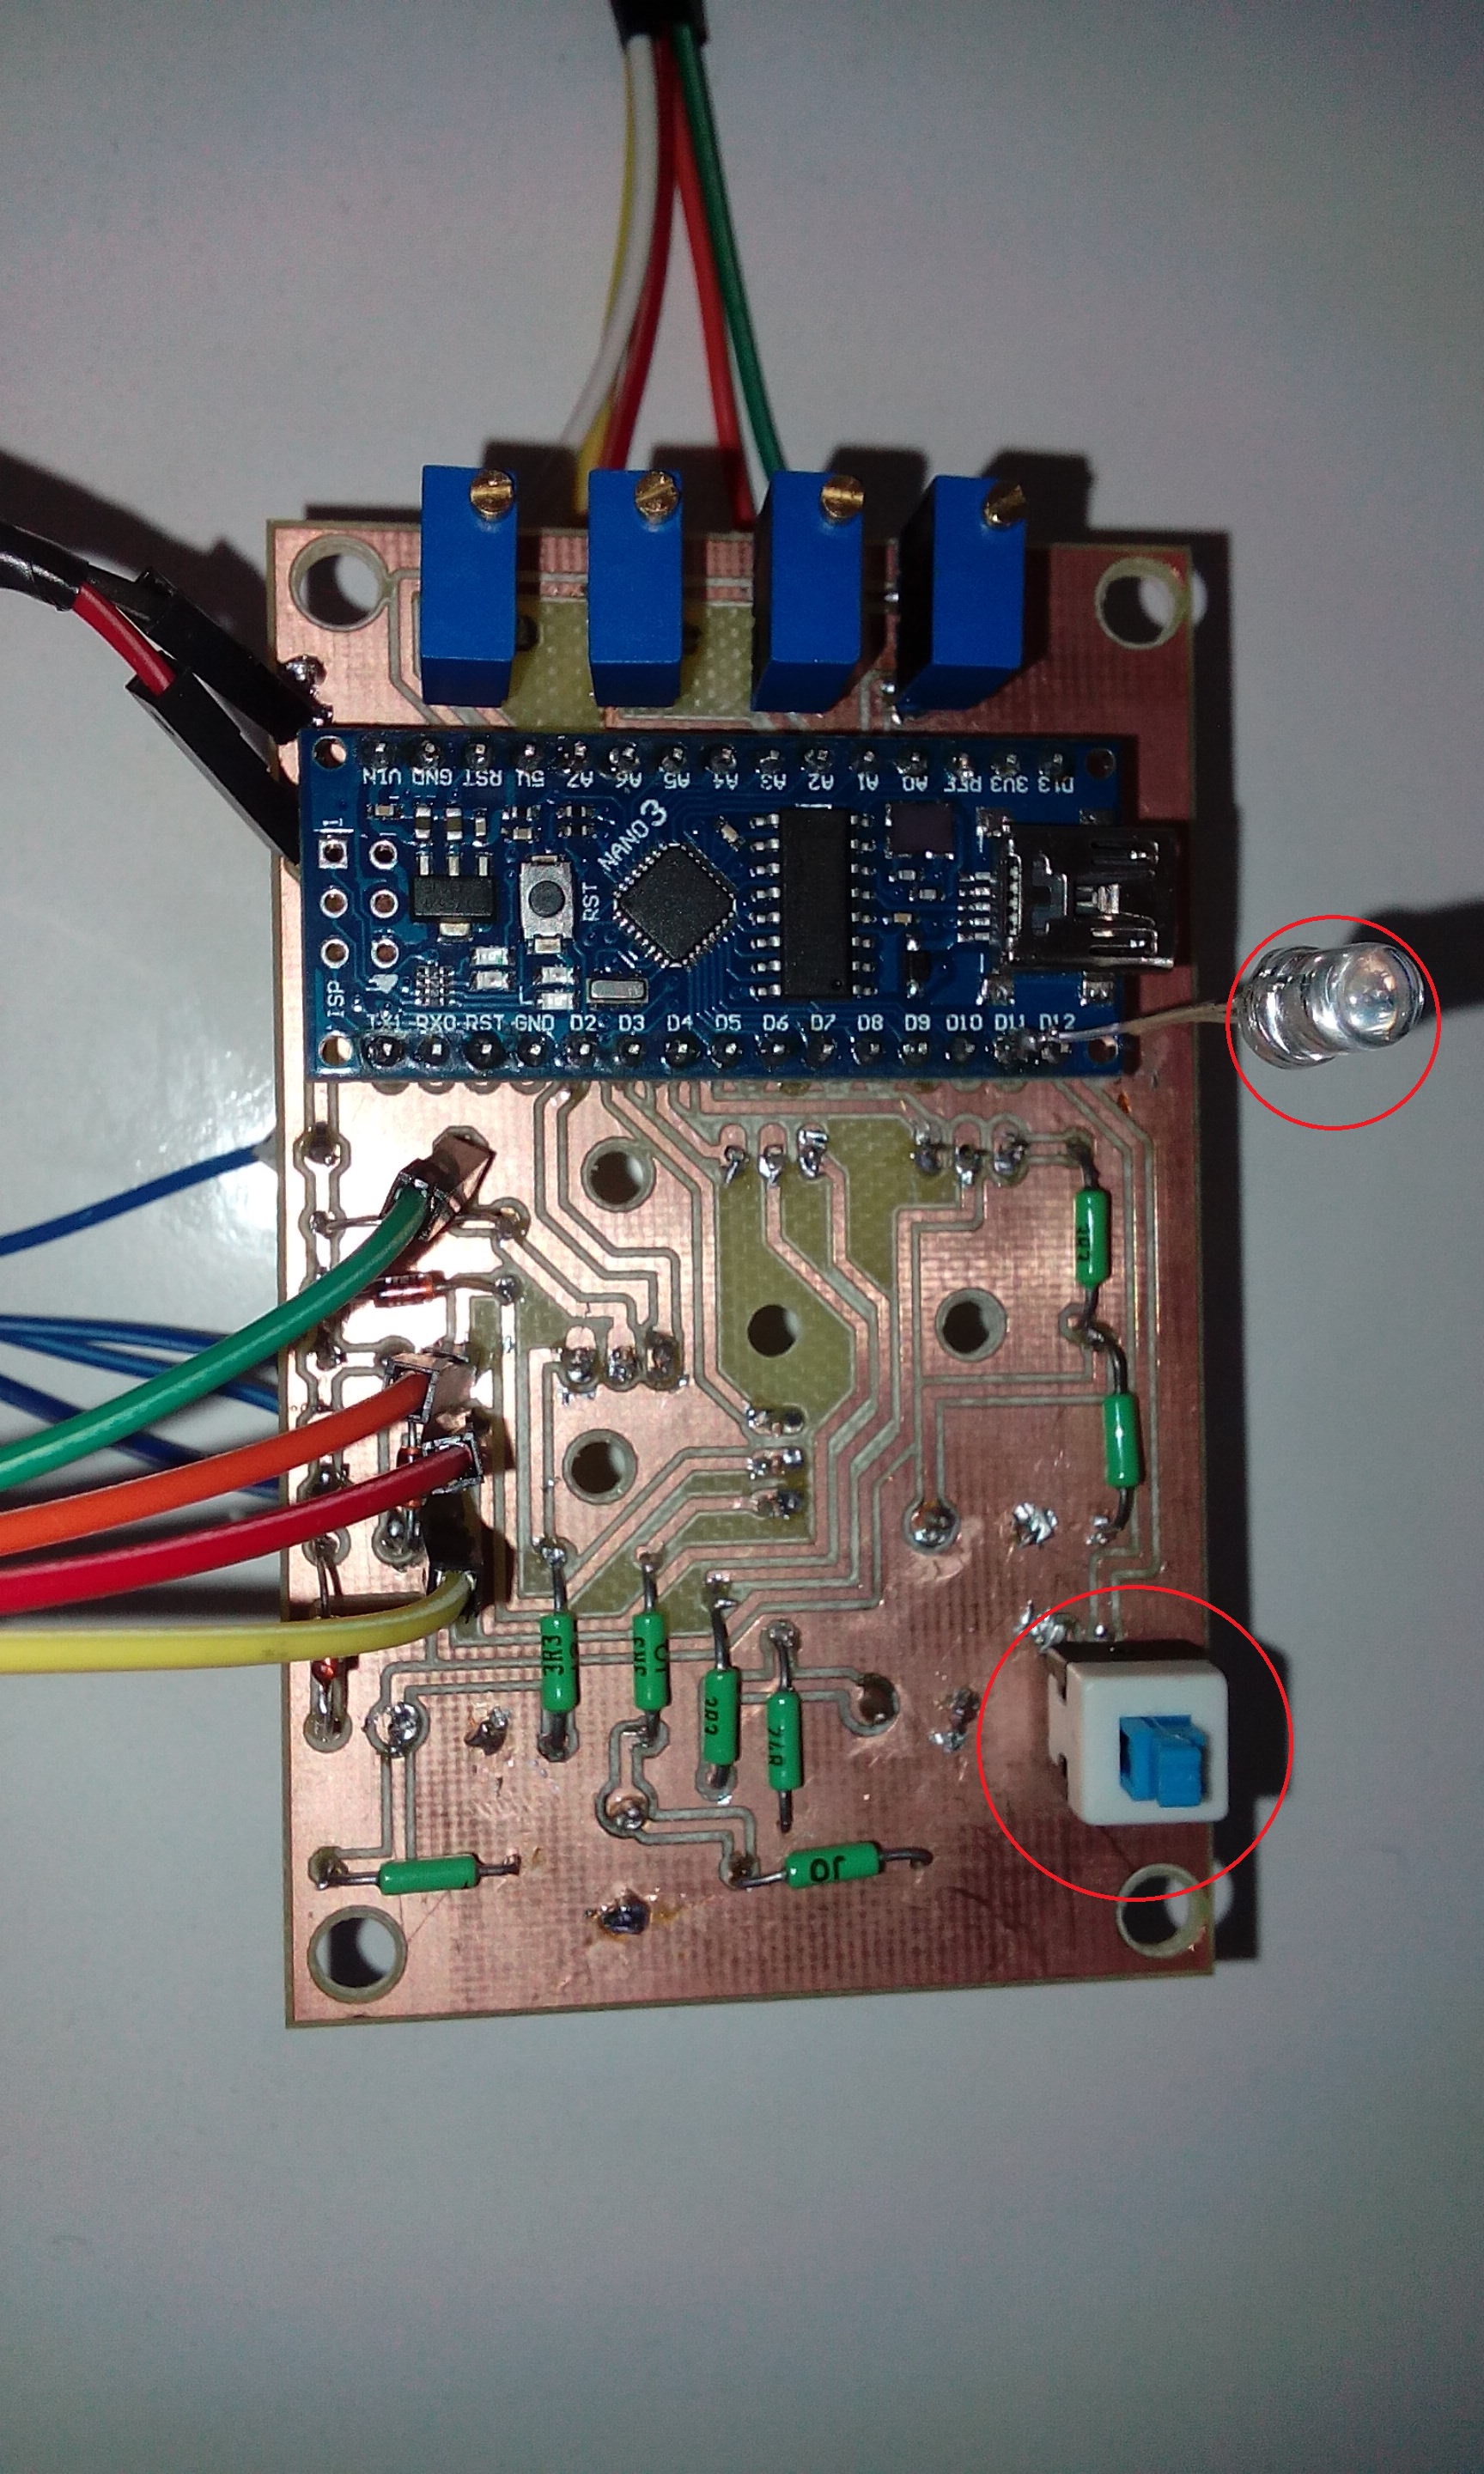
\includegraphics[width=0.70\textwidth]{./img/Navod.jpg}\\[1cm] 
\caption{Fotografie desky plošných spojů s detailem na kontrolní LED diodu a tlačítko}
\label{Navod}
\end{figure}  

\part{Shrnutí a závěr}\label{shrnuti}

\qquad Z hlediska mechanické části projektu se nám podařilo dosáhnout nadočekávané přesnosti. Při sepnutí solenoidů dojde vždy ke stisknutí displaye smartphonu a zároveň, díky možnosti mírného promáčknutí stylusu, nedochází k tomu, že by reakční síla tlačila proti generovanému magnetickému poli. Solenoidy rovněž zvládají spínat i rychlosti, na kterých dochází k chybám snímačů.

\qquad Díky návrhu elektronické části se nám podařilo pomocí zdroje 12V/2A ovládat najednou všechny čtyři solenoidy, a navíc jsme dosáhli i úspory energie (z původně odebíraných 1.1A na solenoid se proud snížil na cca 150mA na solenoid).

\qquad V momentě, kdy je tato dokumentace dotvářena dokáže model hrát hru, běžící rychlostí 10,5 Tiles/s (Světový rekord je 17 Tiles/s). Musíme pamatovat, že největším nedostatkem celého projektu je rychlost FPS smartphonu, na kterém hru hrajeme. Už od 8 Tiles/s jsou obdélníky rozmazané.

\qquad Pokud se k Piano Tales Masterovi ještě v budoucnu vrátíme určitě by jsme rádi vylepšili detekci delších obdélníkových úseků, upravili kalibraci tak, aby byla netečná k hrubému zacházení s modelem a okolnímu jasu a  doladili program tak, aby zvládal hrát co nejdéle.

\qquad Funkční model Piano Tales Mastera si lze prohlédnou na přiloženém videu (viz. Příloha \hyperref[Prilohy]{7}).

\qquad Poznámka na konec. Skutečný název hry, kterou robot hraje je Piano Tiles 2, avšak v zadání je uveden název Piano Tales. Drželi jsme se tedy striktně názvu uvedeném v zadání.
%%%%%%%%%%%%%%%%%%%%%%%%%%%%%%%%%%%%%%%%%%%%%%%%%%%%%%%%%%%%%%%%%%%%%%%%%%%%%%%%%
%%%%%%%%%%%%%%%%%%%%%%%%%%%%%%%%%%%%%%%%%%%%%%%%%%%%%%%%%%%%%%%%%%%%%%%%%%%%%%%%%
%%%%%%%%%%%%%%%%%%%%%%%%%%%%%%%%%%%%%%%%%%%%%%%%%%%%%%%%%%%%%%%%%%%%%%%%%%%%%%%%%
%%%%%%%%%%%%%%%%%%%%%%%%%%%%%%%%%%%%%%%%%%%%%%%%%%%%%%%%%%%%%%%%%%%%%%%%%%%%%%%%%
\part{Přílohy a zdroje}\label{Pril_zdr}

\chapter{Přílohy}\label{Prilohy}

(1) Mechanická část - Návrh modelu v prostředí Autocad a nákresy jednotlivých částí v pdf\\
(2) Deska plošných spojů - Vytvořená v prostředí Eagle (přiloženo včetně schématu)\\
(3) Řídící obvod - Návrh v prostředí Matlab Simulink a spouštěcí m-file\\
(4) Datasheety - Přiložené datasheety pro elektronické komponenty\\
(5) Zdrojové kódy dokumentace v Latexu\\
(6) Zdrojové kódy řídícího programu\\
(7) Video demonstrující funkčnost modelu


\begin{thebibliography}{9}

\bibitem{grabcad} 
GRABCAD COMMUNITY,
\textit{3D model použitého solenoiu}
\\\texttt{https://grabcad.com/library/tag/rob-11015}

\bibitem{latex} 
Overleaf,
\textit{Návody k prostředí \LaTeX\ }
\\\texttt{https://www.overleaf.com/learn}

\bibitem{mathworks} 
MathWorks,
\textit{Návody k prostředí Matlab }
\\\texttt{https://www.mathworks.com/}

\bibitem{solenoid_bib} 
SCIENCING,
\textit{Článek popisující princip funkce solenoidu}
\\\texttt{https://sciencing.com/a-solenoid-work-4567178.html}

\bibitem{robotika} 
Robotika,
\textit{Web předmětu Robotika, navštěvovaný zejména kvůli návodům k gitu}
\\\texttt{https://sites.google.com/site/vutrobotika/home}

\end{thebibliography}
\end{document}
